\begin{question}
\noindent A space mission planner is designing a symmetrical logo for a satellite launch. The design team draws triangle $E$ on a coordinate grid to represent one half of the emblem, as shown below.

\begin{center}
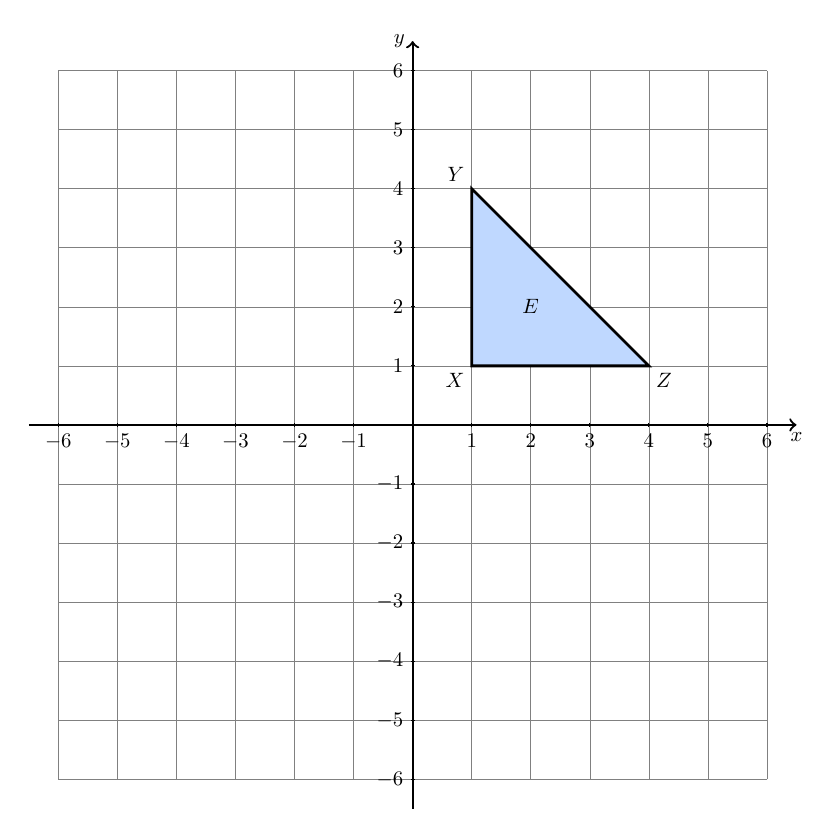
\begin{tikzpicture}[scale=0.75, transform shape]
    \definecolor{borderColour}{HTML}{000000}
    \definecolor{fillColourE}{HTML}{BFD8FF}

    \def\axisLimit{6}

    % Draw grid
    \draw[step=1cm,gray,very thin] (-\axisLimit,-\axisLimit) grid (\axisLimit,\axisLimit);

    % Draw axes
    \draw[thick,->] (-\axisLimit-0.5,0) -- (\axisLimit+0.5,0) node[anchor=north] {$x$};
    \draw[thick,->] (0,-\axisLimit-0.5) -- (0,\axisLimit+0.5) node[anchor=east] {$y$};

    % Label x-axis and y-axis
    \foreach \x in {-\axisLimit,...,-1,1,2,...,\axisLimit}
        \draw (\x cm,1pt) -- (\x cm,-1pt) node[anchor=north] {$\x$};
    \foreach \y in {-\axisLimit,...,-1,1,2,...,\axisLimit}
        \draw (1pt,\y cm) -- (-1pt,\y cm) node[anchor=east] {$\y$};

    % Triangle E: vertices X(1,1), Y(1,4), Z(4,1)
    \coordinate (X) at (1,1);
    \coordinate (Y) at (1,4);
    \coordinate (Z) at (4,1);
    \filldraw[fill=fillColourE, draw=borderColour, line width=1pt] (X) -- (Y) -- (Z) -- cycle;

    \node[below left] at (X) {$X$};
    \node[above left] at (Y) {$Y$};
    \node[below right] at (Z) {$Z$};
    \node at (2,2) {$E$};

\end{tikzpicture}
\end{center}

\noindent Reflect triangle $E$ in the $y$-axis.

Draw and label the image triangle $E'$ on the grid, showing the coordinates of each vertex clearly.

\vspace{4cm}

\begin{flushright}
    \answerplain{2}
\end{flushright}
\end{question}